\documentclass[12pt,twoside]{article} 
\usepackage{amsmath, amssymb} 
\usepackage{graphicx}
\usepackage{amsmath} 
\usepackage[active]{srcltx} 
\usepackage{amssymb} 
\usepackage{amscd} 
\usepackage{makeidx} 
\usepackage{amsthm} 
\usepackage{algpseudocode} 
\usepackage{algorithm}
\usepackage[spanish, activeacute]{babel}
\usepackage[utf8]{inputenc}

\renewcommand{\baselinestretch}{1}
\setcounter{page}{1}
\setlength{\textheight}{21.6cm}
\setlength{\textwidth}{14cm}
\setlength{\oddsidemargin}{1cm}
\setlength{\evensidemargin}{1cm}
\pagestyle{myheadings}
\thispagestyle{empty}
\markboth{\small{Pr\'actica 1. Fernando Rivera, Alejandro Contreras.}}{\small{.}}
\date{}
\begin{document}
\centerline{\bf An\'alisis de Algoritmos, Sem: 2020-1, 3CV2, Pr\'actica 1, 21/08/2019 } \centerline{}
\centerline{}
\begin{center}
\Large{\textsc{Pr\'actica 1: Determinaci\'on experimental de la complejidad temporal de un algoritmo}}
\end{center}
\centerline{}
\centerline{\bf {Rivera Paredes Fernando Daniel, Contreras Paredes Alejandro.}}
\centerline{}
\centerline{Escuela Superior de C\'omputo}
\centerline{Instituto Polit\'ecnico Nacional, M\'exico}
\centerline{$ferny036@hotmail.com, acontrerasparedes@hotmail.com$}
\newtheorem{Theorem}{\quad Theorem}[section] \newtheorem{Definition}[Theorem]{\quad Definition} \newtheorem{Corollary}[Theorem]{\quad Corollary} \newtheorem{Lemma}[Theorem]{\quad Lemma} \newtheorem{Example}[Theorem]{\quad Example} \bigskip
\textbf{Resumen:} Se plantea definiciones principales sobre complejidad en el desarrollo de los algoritmos. Hablamos un poco acerca de las definiciones sobre
notaciones de complejidad, planteamos dos problema diferentes y verificamos su comportamiento a trav\'es del uso de gr\'aficas.

\centerline{}
{\bf Palabras Clave:} Fibonacci, Euclides, MCD, Complejidad, Grafica
\newpage
\section{Introducci\'on}
Está práctica es realizada para reforzar los conocimientos obtenidos en clase, así como, para desarrollar en tiempo real las 
habilidades de cursos anteriores y combinarlas con el análisis de algoritmos, Esto por su parte es para llegar a la resolución de varios 
problemas que fueron planteados para la realización de la práctica.
Ya teniendo el conocimiento de los algoritmos planteados, se procedió a la codificación de estos, se utilizaron dos entornos diferentes,
C y Python.
Una vez codificados, se les agrego una manera de contabilizar cuál es su costó computacional y ver en qué magnitud se rigen los 
algoritmos para después realizar sus gráficas y comparar los resultados obtenidos con lo teórico y lo esperado.
Finalmente el objetivo es plantear una solución a problemas dados y comprobar que estos son cuan lo menos parecido a los resultados vistos en clase.
\section{Conceptos B\'asicos} 
\subsection{\textbf{Complejidad Computacional}}
\setlength{\parindent}{1.5em}
Podemos hablar de complejidad computacional a la rama que estudia el orden de complejidad de un algoritmo que 
resuelve un problema decidible. Para ello, considera los 2 Dpos de recursos requeridos durante el cómputo para resolver un problema:
\begin{itemize}
  \item Tiempo: Número de pasos base de ejecución de un algoritmo para resolver un problema.
  \item Espacio: Cantidad de memoria utilizada para resolver un problema.

\end{itemize}

La complejidad de un algoritmo se expresa como función del tama\~no de la entrada del problema, n.
Se refiere al ratio de crecimiento de los recursos con respecto a n:
\begin{itemize}
  \item Ratio del Tiempo de ejecución (Temporal): T(n).
  \item Ratio del espacio de almacenamiento necesario (Espacial): S(n).
\end{itemize}
\centerline{}
\subsection{\textbf{Clasificaci\'on de Problemas de desici\'on}}
\setlength{\parindent}{1.5em}

Las clases de problemas de decisión son:
\begin{itemize}
  \item Clase P (Polynomial Time): Son todos aquellos problemas de decisión que pueden ser resueltos por una MT determinista en un 
    período de tiempo polinómico. Estos problemas son tratables, es decir se pueden resolver en tiempos razonable; buena parte de 
    los problemas de ordenamiento, priorización y búsqueda caben dentro de esta clase.
  \item Clase NP (Non Deterministic Polynomial Time): Formalmente, es el conjunto de problemas que pueden ser resueltos en tiempo 
    polinómico por una MT no determinista. Una definición más intuitiva es la siguiente: Es el conjunto de los problemas de 
    decisión para los cuales las instancias donde la respuesta es “si” tienen demostraciones verificables por cálculos 
    determinísticos en tiempo polinómico. La importancia de esta clase de problemas es que es aplicable cuando se desea saber
    si existe una cierta solución o si existe una mejor solución que las conocidas.
  \item Clase NP-Completo: Estos problemas son NP, sus soluciones sus soluciones son reducibles a NP en tiempo polinómico.

\end{itemize}

Nadie, hasta ahora, ha podido demostrar en forma concluyente que todos los problemas NP-Completos se pueden resolver dentro de 
tiempos polinomiales, esto ha creado una de las grandes discusiones científicas al punto que el Instituto Clay de Matemáticas 
definió este como como uno de los siete problemas insolubles y ofrece para quien lo demuestre una recompensa de US 1.000.000.

\subsection{\textbf{Notaci\'on $\Theta$ }}
Una funcion $f(n)$ pertenece al conjunto $\Theta(g(n))$ si existen constantes positivas $C_{1}$ y $C_{2}$ tales que pueden ser acotadas 
por $C_{1}g(n)$ y $C_{2}g(n)$ \(tanto por arriba como por abajo\) para una n lo suficiente grande. A este tipo de asociaci\'on lo denotamos como:
\begin{center}
  $f(n) \in$ $\Theta (g(n))$
\end{center}
En un sentido mas literal, podemos definir la notaci\'on $\Theta$ de una manera mas formal como:
\begin{center}
  $\Theta(g(n))$ = \{$f(n)$ : $\exists$ $C_{1}$, $C_{2}$, $n_{0}$ $\ge$ 1 tales que $C_{1}$
  $ g(n) \leq f(n) \leq C_{2}$ $g(n)$, $\forall n \ge n_{0}$\}
\end{center}

\subsection{\textbf{Notaci\'on $O$ }}
Una funcion $f(n)$ pertenece al conjunto $O(g(n))$ si existe una constante positivas $C$ tal que puede ser acotada 
por arriba por $C\cdot g(n)$ para una n lo suficiente grande. A este tipo de asociaci\'on lo denotamos como:
\begin{center}
  $f(n) \in$ $O(g(n))$
\end{center}
En un sentido mas literal, podemos definir la notaci\'on $O$ de una manera mas formal como:\\
\begin{center}
  $O(g(n))$ = \{$f(n)$ : $\exists$ $C$, $n_{0}$ $\ge$ 1 tal que 
$ 0 \leq f(n) \leq C \cdot g(n)$, $\forall n \ge n_{0}$\}
\end{center}

\subsection{\textbf{Notaci\'on $\Omega$ }}
Una funcion $f(n)$ pertenece al conjunto $\Omega (g(n))$ si existe una constante positivas $C$ tal que puede ser acotada 
por arriba por $C\cdot g(n)$ para una n lo suficiente grande. A este tipo de asociaci\'on lo denotamos como:
\begin{center}
  $f(n) \in$ $\Omega (g(n))$
\end{center}
En un sentido mas literal, podemos definir la notaci\'on $O$ de una manera mas formal como:
\begin{center}
  $\Omega (g(n))$ = \{$f(n)$ : $\exists$ $C$, $n_{0}$ $\ge$ 1 tal que 
$ 0 \leq f(n) \leq C \cdot g(n)$, $\forall n \ge n_{0}$\}
\end{center}
\section{Experimentaci\'on y Resultados}
\subsection{\textbf{Planteamiento de los distintos problemas}}
Al desarrollo de la pr\'actica tenemos planteado resolver 2 problemas completamente distintos.El primero tiene que ver con
una suma binaria, donde el tamaño del numero binario viene denotado como:
\begin{center}
  $k = \log_{2}n$ $\Rightarrow$ $n = 2^k$
\end{center}
Por lo que se tendria que determinar el costo para cada valor de $n$ respecto a $k$, tenien en cuenta que en la suma binaria
puede producir un resultado con tamaño $n + 1$.

\centerline{}
Para el segundo problema tenemos que desarrollar el algoritmo de euclides para el calculo del M\'aximo Com\'un Divisor (MCD), 
sin embargo tiene una condici\'on especial donde hay que determinar el MCD de 2 n\'umeros de la sucesion de Fibonacci tales que 
sean los \'ultimos con la misma cantidad de digitos, por ejemplo, el $89$ y el $55$ son el \'ultimo par con 2 digitos, por lo tanto,
se este par se determinara el valor del MCD entre estos.
\subsection{\textbf{Soluci\'on al primer problema}}
Este primer programa lo programamos en python, en principio creamos 3 listas que al final 2 de estas tienen el mismo tamaño, y la 
\'ultima podr\'ia cambiar su tama\~no. Creamos una funci\'on $iniciarListas()$, que permit\'ia claramente, inicializar las listas,
donde en cada uno de sus campos se les asigna aleatoriamente con 0's o 1's, posteriormente en una funci\'on, realizamos la dedicada
suma binaria de acuerdo a su mapa l\'ogico de circuitos, donde el siguiente valor en el resultados era una operaci\'on l\'ogica de 
$xor$, entre estas operaciones se encuentra una variable auxiliar que funciona como corrimiento en la suma de bits, y por supuesto,
tambien calculamos el valor que obtendria esta variable auxiliar para utilizarla en la siguiente operaci\'on $xor$.
\centerline{}
Para cada valor de $k$ entre $[1..m]$, consideramos $m = 10$ como m\'aximo valor en $k$ para el n\'umero 
de elementos en la suma binaria. Este fue el resultado con vista hasta k = 5.$(Figura$ $1)$.
\begin{figure}
  \centering
    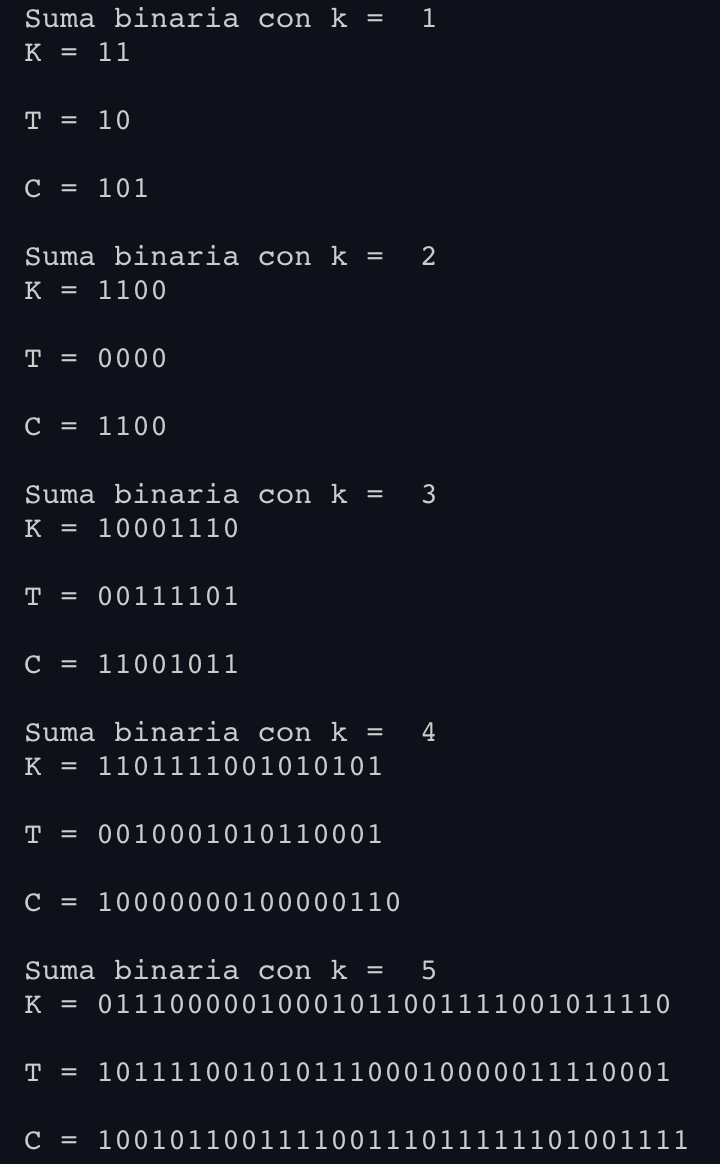
\includegraphics[height=0.5\textwidth]{Figure1}
  \caption{Resultados aleatorios con k desde 1 hasta 6}
  \label{fig:ejemplo1}
\end{figure}

Para ver el comportamiento del algortimo respecto a los ``costos'' que genera realizamos una gr\'afica.$(Figura$ $2)$.

\begin{figure}
  \centering
    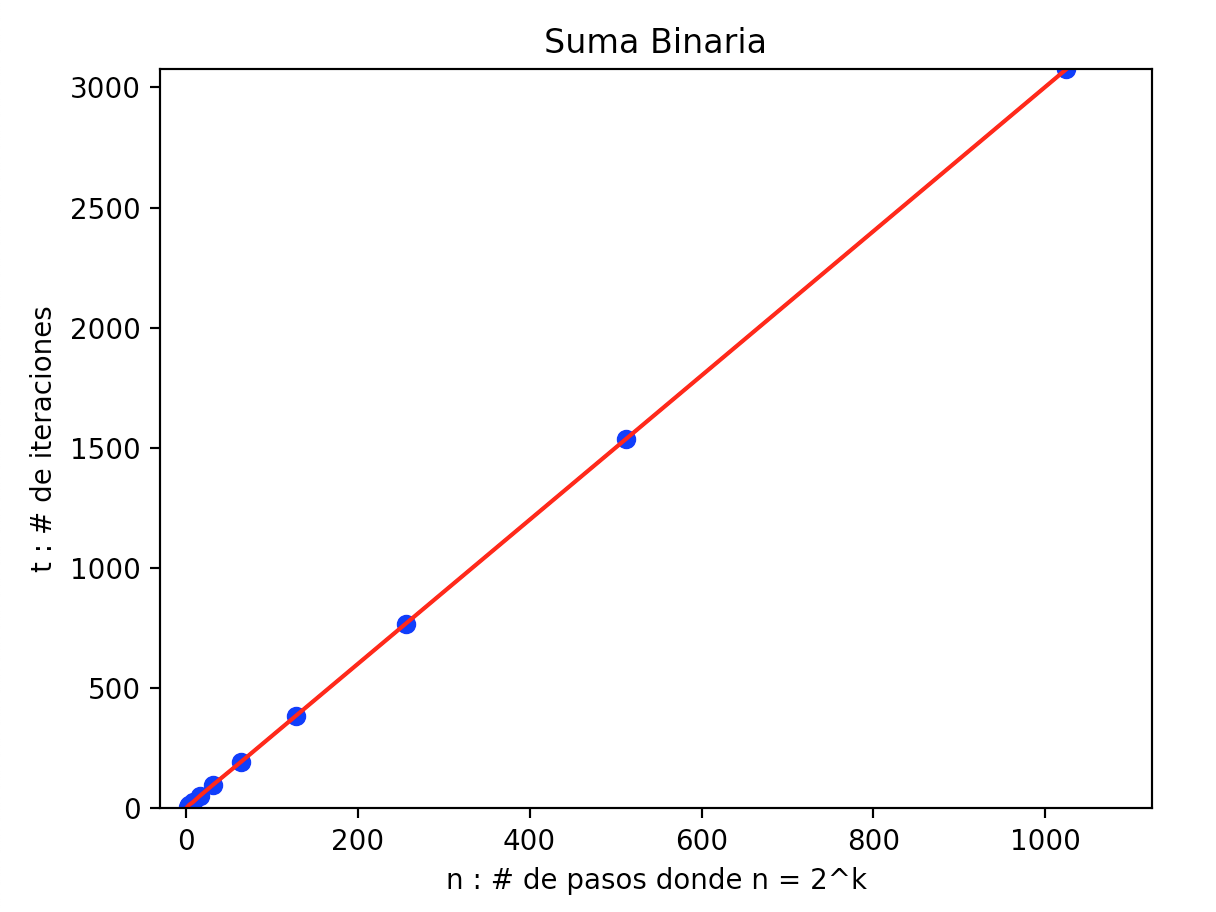
\includegraphics[height=0.5\textwidth]{Figure2}
  \caption{Gr\'afica del comportamiento de la suma binaria}
  \label{fig:ejemplo2}
\end{figure}

\subsection{\textbf{Soluci\'on al segundo problema}}
En el segundo problema, para no perder el ritmo a lo aprendido, lo decidimos programarlo en lenguaje C, donde aplicamos tanto el
algoritmo de Esclides, como Fibonacci, de tal forma que en el algoritmo de Fibonacci nos pudiese obtener los valores deseados,
que son n\'umeros sucesivos de Fibonacci con la misma cantidad de d\'igitos, estos almacenarlos en un array, el cual ser\'a
recorrido en pares para calcular su MCD, y determinar los costos para ese algoritmo en especifico.
De tal forma que obtuviera todos los pares con la misma cantidad de digitos entre los numeros que se pueden obtener en lenguaje C,
el cual nos permiti\'o trabajar con el tipo de dato $unsigned long long int$, aunque las tablas de resultados no se imprimieron como
esper\'abamos, dieron con todos los resultados que esper\'abamos $(Figura$ $3)$.

\begin{figure}
  \centering
    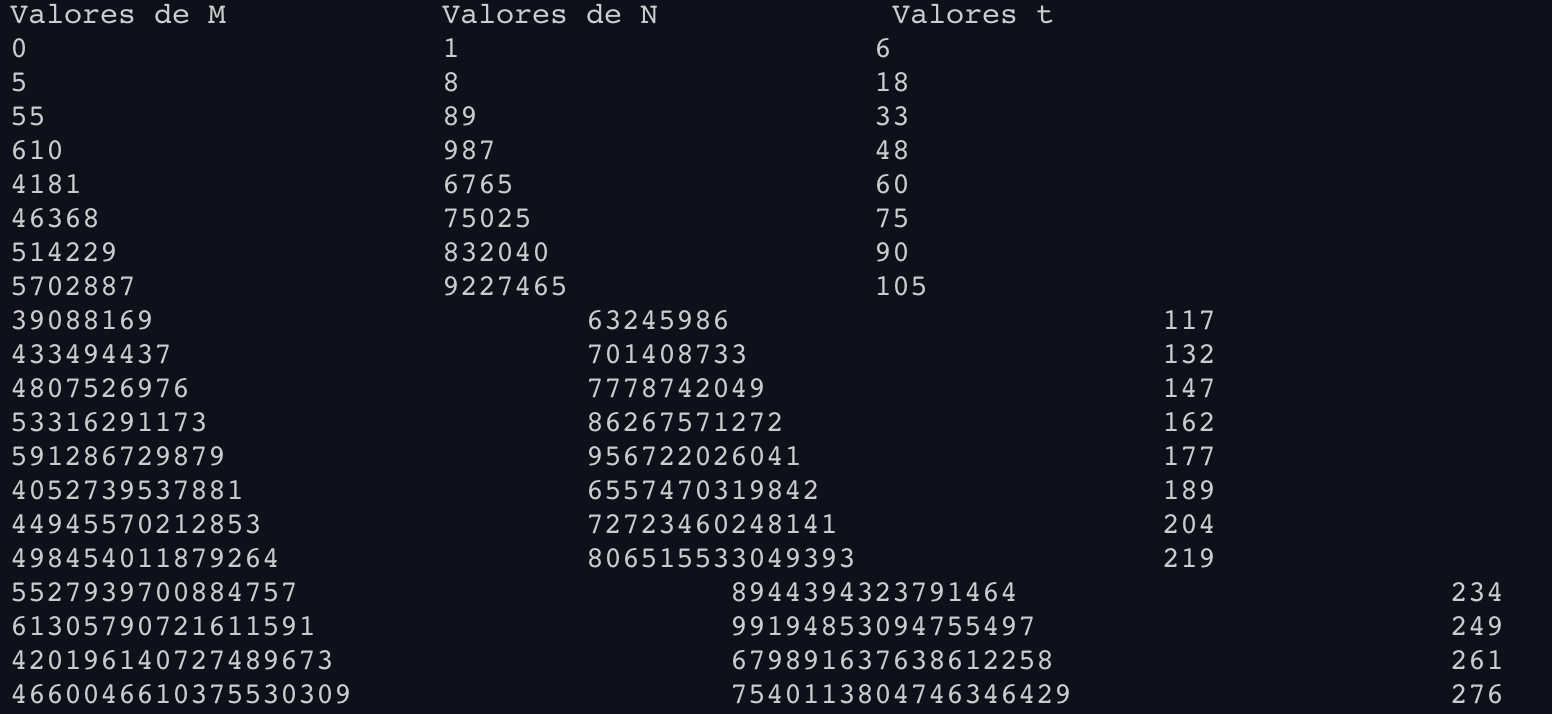
\includegraphics[height=0.5\textwidth]{Figure3}
  \caption{Prueba de Escritorio Respecto a m y n}
  \label{fig:ejemplo3}
\end{figure}

\begin{figure}
  \centering
    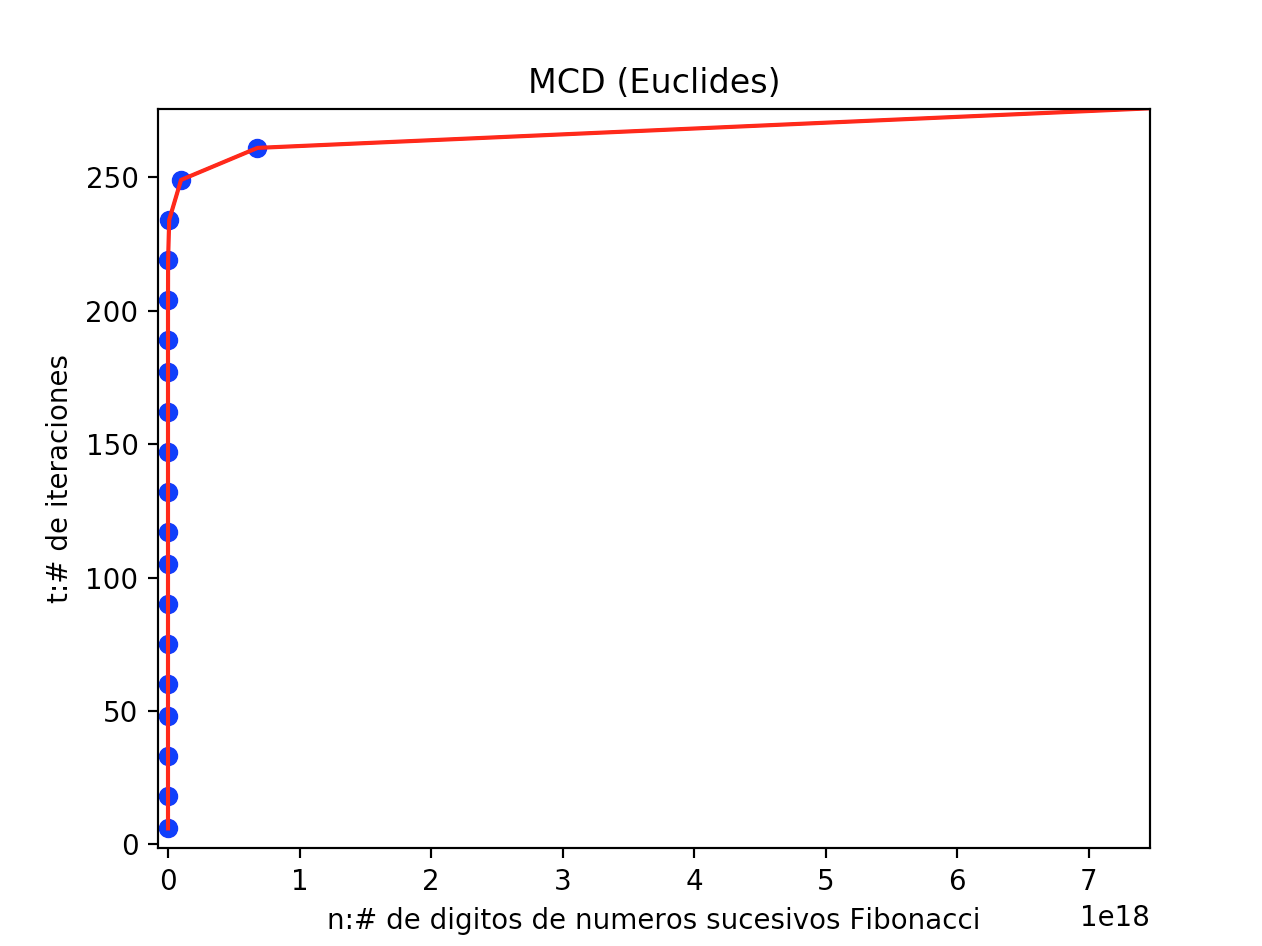
\includegraphics[height=0.5\textwidth]{Figure4}
  \caption{Gr\'afica del segundo problema, Euclides}
  \label{fig:ejemplo4}
\end{figure}
\newpage

\section{Anexo} 
\text{}\\ 
\textbf{Cálculo del orden de complejidad del
algoritmo Select-sort}\\ 
\text{El peor de los casos es cuando el arreglo esta acomodado de forma descendente.}\\ 

\begin{center}
  \begin{tabular}{ l | c }
    Costo & No. de Veces\\ \hline
    C1 & $n$ \\
    C2 & $n-1$ \\ 
    C3 & $\sum_{j=0}^{n-2}t_{j}$ \\
    C4 & $\sum_{j=0}^{n-2}(t_{j}-1)$ \\
    C5 & $\sum_{j=0}^{n-2}(t_{j}-1)$ \\ 
    C6 & $n-1$ \\
  \end{tabular}
\end{center}
Analizando el comportamiento en el peor de los casos se obtiene:\\
\[\Rightarrow T(n) = C_{1}n + C_{2}(n-1) + 
C_{3}\sum_{j=0}
^{n-2}t_{j} +  
C_{4}\sum_{j=0}^{n-2}(t_{j}-1) +
C_{5}\sum_{j=0}^{n-2}(t_{j}-1) + C_{6}(n-1)\] 
donde:
\begin{center}
  \begin{tabular}{ l | c }
    j & $t_{j}$\\ \hline
    0 & $n$ \\
    1 & $n-1$ \\ 
    2 & $n-2$ \\
    . & . \\
    . & . \\ 
    n & $n-j$ \\
  \end{tabular}
\end{center}
Para calcular la complejidad en el peor de los casos debemos multiplicar
el costo y el numro de veces que es ejutado el codigo por linea, lo cual queda de la siguiente manera:
\[\Rightarrow T(n) = C_{1}n + C_{2}(n-1) + 
C_{3}\sum_{j=0}^{n-2}(n-j) +  
C_{4}\sum_{j=0}^{n-2}(n-j-1) +
C_{5}\sum_{j=0}^{n-2}(n-j-1) + C_{6}(n-1)\] 
Si se despeja $n$ algebraicamente tenemos:
\begin{center}
\[\Rightarrow T(n) = C_{1}n + C_{2}(n-1) + 
C_{3}\sum_{j=0}^{n-2}n -
C_{3}\sum_{j=0}^{n-2}j +  
C_{4}\sum_{j=0}^{n-2}n -
C_{4}\sum_{j=0}^{n-2}j -\]\[
C_{4}\sum_{j=0}^{n-2}1 +
C_{5}\sum_{j=0}^{n-2}n -
C_{5}\sum_{j=0}^{n-2}j - 
C_{5}\sum_{j=0}^{n-2}1 + 
C_{6}(n-1)\]
\end{center}

\[\Rightarrow T(n) = (C_{1} + C_{2} + C_{6})n - C_{2} +  
C_{4}(n-1)n + 
C_{4}\frac{(n-1)(n-2)}{2} - C_{4}(n-1) +\]\[
C_{5}(n-1)n -  
C_{5}\frac{(n-1)(n-2)}{2} - C_{5}(n-1)n - 
C_{5}\]


\[\Rightarrow T(n) = (\frac{C_{4}}{2} + C_{4} + C_{5} + \frac{C_{5}}{2})n^{2} + \]\[
(C_{4} + C_{2} + C_{6} - C_{4} + \frac{3C_{4}}{2} - C_{4} + C_{5} + \frac{3C_{5}}{2} -C_{5})n +\]\[
(- C_{2} - C_{4} + C_{4} + C_{5} - C_{5} - C_{6})\]

\[\Rightarrow T(n)= an^2 +bn + c\]

\[\therefore T(n) \in O(n^2) \]
\newpage
\section{Conclusiones}
\textbf{Conclusion Alejandro Contreras Paredes}\\

Como primera práctica, resulta algo confusa por no tener aun bien cimentados 
los fundamentos del analisis de algoritmos pero a su vez es enriquesedor poner en uso 
los conocimientos teoricos que fueron dados ya clases atras. Puedo decir que resulta interesante 
como estan relacionados el costo computacional con la complejidad derivada de un algoritmo, el calculo del costo
no resulta complejo porque depende memaremnte de la estructura con la que fue programado el algoritmo. Entonces
como aun no se eleva el grado de complejidad de los algoritmos, puedo concluir que esta practica fue realizada 
hasta donde nuestras capacidades nos dieron a entender, poniendo un esfuerzo y dedicación.
\\\\
\textbf{Conclusion Fernando Daniel Rivera Paredes}\\

Con esta practica aprendimos lo escencial para ver como funciona un algoritmo a nivel te\'orico, el cual nos
permite ver un nuevo panorama nuevo respecto a las materias que habiamos llevado anteriormente, todo esto con 
su grado de dificultad para que se lleve bien a cabo, tanto en ver la optimizaci\'on o ahorro de recursos, como 
lo vimos, tanto de tiempo como de almacenamiento, creamos un algoritmo de complejidad baja para los casos 
especiales solicitados, que por tanto, fue muy buen algoritmo, el cual nos permitio utilizar poca memoria, y su 
ejecuci\'on fue ampliamente r\'apida. Espero para las siguientes pr\'acticas sean similares o peores, en el sentido
del nivel de dificultad.
\begin{figure}[!h]
	\centering
	\begin{minipage}[t]{10cm}
		\centering
		
\includegraphics[scale=0.2]{Foto1}
		\caption{Alejandro Contreras Paredes}
	\end{minipage}
	\hspace{18cm}
	\begin{minipage}[t]{10cm}
		\centering
		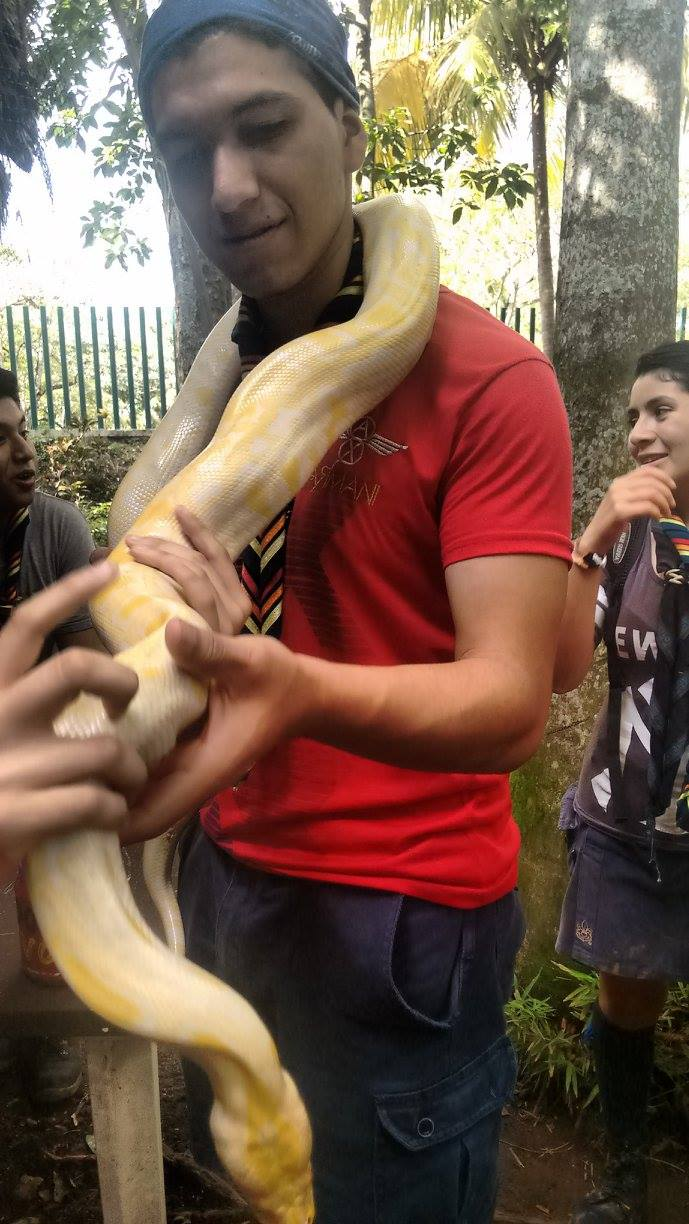
\includegraphics[scale=0.2]{Foto2}
		\caption{Rivera Paredes Fernando Daniel}
	\end{minipage}
\end{figure}

\section{Bibliograf\'ia}

\begin{thebibliography}{9}
  \bibitem{book} 
  Cormen, T. and Leiserson, C.
  \textit{Introduction to algorithms.} 
  3rd edition.Cambridge, Massachusetts: Massachusetts Institute of Technology, 2009.

  \bibitem{ie} 
  Moyano, N.
  \textit{¿Qué es la Complejidad Computacional?.}.
  Medium. Available at: https://medium.com/@nelramoyano/qué-es-la-complejidad-computacional-3a556e557973.'[Accessed 22 Aug. 2019].
\end{thebibliography}
\end{document}